
Since tenants pay based on the time they occupy their
VMs, and this time is influenced by the network, tenants
implicitly end up paying for the network traffic; yet, such
communication is supposedly free (hidden cost).

\subsection{Virtual Network Abstractions}

The “virtual” nature of the network implies that the provider
has a lot of freedom in terms of the topology of this
network, and can offer different options to tenants for different
costs. Beyond the overarching goal of maintaining the
simplicity of the interface between tenants and providers,
our topologies or virtual network abstractions are guided by
two design goals:

\begin{description}
\item[Tenant suitability] The abstractions should allow tenants
to reason in an intuitive way about the network performance
of their applications when running atop the virtual
network.
\item[Provider flexibility] Providers should be able to multiplex
many virtual networks on their physical network.
The greater the amount of sharing possible, the lesser
the tenant costs.
\end{description}

To this effect, we propose two novel abstractions for virtual
networks in the following sections.

\subsubsection{Virtual Cluster}

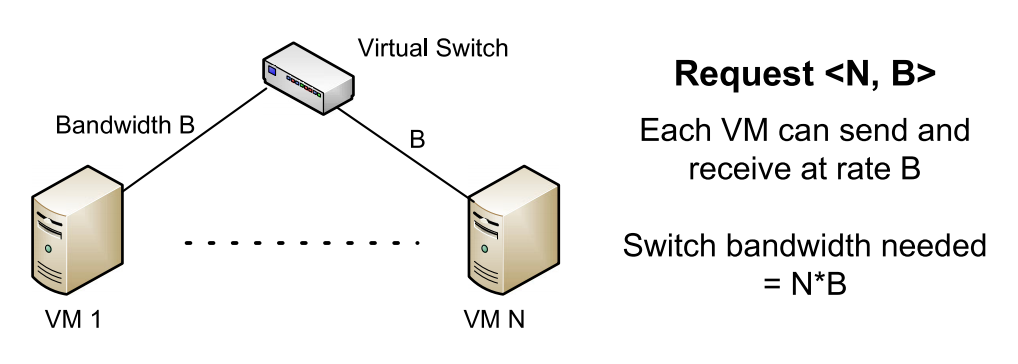
\includegraphics[width=0.8\linewidth]{img/virt_switch.png}

With a virtual cluster, a tenant request
<N, B> provides the following topology: each tenant
machine is connected to a virtual switch by a bidirectional
link of capacity B, resulting in a one-level tree topology. The
virtual switch has a bandwidth of $N \times B$. This ensures that
the virtual network has no oversubscription and the maximum
rate at which the tenant VMs can exchange data is
N ∗ B. However, this data rate is only feasible if the communication
matrix for the tenant application ensures that each VM sends and receives at rate B. Alternatively, if all N
tenant VMs were to send data to a single destination VM,
the data rate achieved will be limited to B.
Since a virtual cluster offers tenants a network with no
oversubscription, \textbf{it is suitable for data-intensive applications
like MapReduce and BLAST}. For precisely such applications,
Amazon’s Cluster Compute provides tenants with
compute instances connected through a dedicated 10 Gbps
network with no oversubscription. This may be regarded as
a specific realization of the virtual cluster abstraction with
<N , 10 Gbps>.

\subsubsection{Virtual Oversubscribed Cluster}

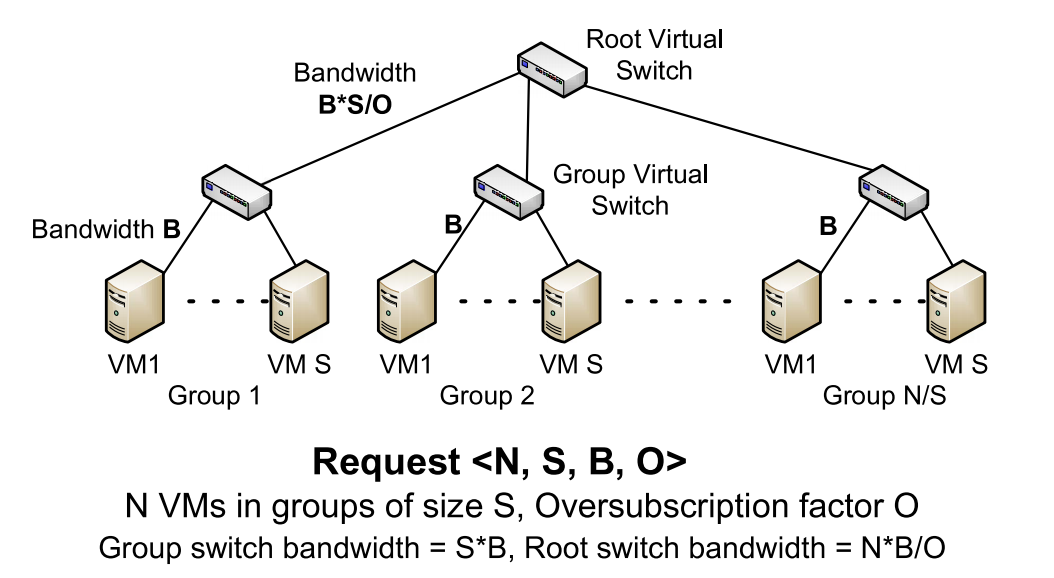
\includegraphics[width=0.8\linewidth]{img/virt_over_subscribed.png}

While a network with no oversubscription is imperative
for data-intensive applications, this does not hold for many
other applications [19,34]. Instead, a lot of cloud bound applications
are structured in the form of components with
more intra-component communication than inter-component
communication [16,25]. A “Virtual Oversubscribed Cluster”
is better suited for such cases; it capitalizes on application
structure to reduce the bandwidth needed from the underlying
physical infrastructure compared to virtual clusters,
thereby improving provider flexibility and reducing tenant
costs.

With a virtual oversubscribed cluster, a tenant request
<N , B, S, O>. Tenant
machines are arranged in groups of size S, resulting in $\frac{n}{s}$ groups. VMs in a group are connected by bidirectional links
of capacity $B$ to a (virtual) group switch. The group switches
are further connected using a link of capacity $B' = \frac{S \times B}{O}$ 
to a (virtual) root switch. The resulting topology has no oversubscription
for intra-group communication. However, intergroup
communication has an oversubscription factor $O$, i.e.,
\textbf{the aggregate bandwidth at the VMs is $O$ times greater than
the bandwidth at the root switch}. Hence, this abstraction
closely follows the structure of typical oversubscribed datacenter
networks. Note, however, that $O$ neither depends upon
nor requires physical topology oversubscription. Compared to virtual cluster, this abstraction does not offer
as dense a connectivity. However, the maximum data rate
with this topology is still $N \times B$.

The localized nature of the
tenant’s bandwidth demands resulting from this abstraction
allows the provider to fit more tenants on the physical network.
This, as our evaluation shows, has the potential to
significantly limit tenant costs. By incentivizing tenants to
expose the flexibility of their communication demands, the abstraction achieves better multiplexing which benefits both
tenants and providers. Amazon’s EC2 Spot Instances is
a good example of how tenants are willing to be flexible, especially
when it suits their application demands, if it means
lowered costs.

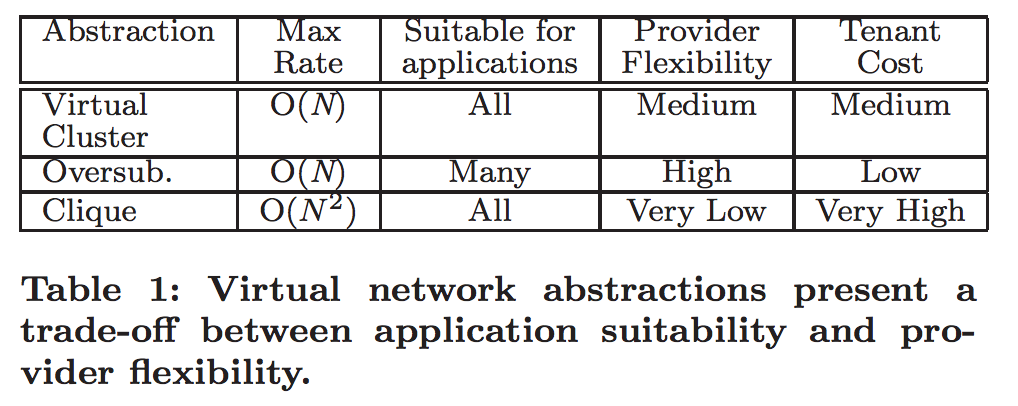
\includegraphics[width=0.7\linewidth]{img/net_comp.png}

\subsection{Oktopus}

With Oktopus,
tenants requesting VMs can opt for a (virtual) cluster or a
(virtual) oversubscribed cluster to connect their VMs.

 Two main components are used:

 \begin{description}
 \item[Management plane] A logically centralized network manager
(NM), upon receiving a tenant request, performs
admission control and maps the request to physical machines.
This process is the same as today’s setup except
that the NM needs to further account for network resources
and maintain bandwidth reservations across the
physical network.
\item[Data plane] Oktopus uses rate-limiting at endhost hypervisors
to enforce the bandwidth available at each VM.
This ensures that no explicit bandwidth reservations at
datacenter switches are required.
 \end{description}

 The network manager implements allocation algorithms
to allocate slots on physical machines to tenant requests in
an online fashion. For tenant requests involving a virtual
network, the NM needs to ensure that the corresponding
bandwidth demands can be met while maximizing the number
of concurrent tenants. To achieve this, the NM maintains
the following information :
\begin{itemize}
\item The datacenter network
topology
\item The residual bandwidth for each link in the
network
\item The empty slots on each physical machine
\item The allocation information for existing tenants,
including the physical machines they are allocated to, the
network routes between these machines and the bandwidth
reserved for the tenant at links along these routes
\end{itemize}

\subsection{End.}

See algorithm in the paper for allocation process, etc.



